% Name: Band gaps
% Description: The electron energy bands of a metal, a semiconductor, and an insulator: filled bands in blue, empty bands outlined, and the gap between them growing from none to small to large.
% Tags: band gap, semiconductor, insulator, metal, solid-state physics

\usetikzlibrary{arrows.meta}

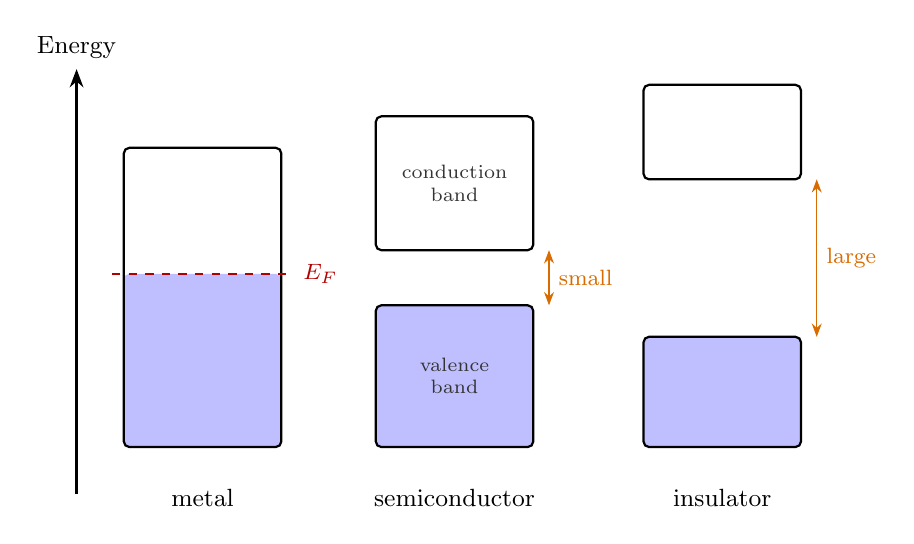
\begin{tikzpicture}[>={Stealth}, every node/.style={font=\small}, band/.style={draw, thick, rounded corners=2pt}]
  \draw[->, thick] (-0.6,-0.2) -- (-0.6,5.2) node[above] {Energy};
  % Metal: one band, filled only up to the Fermi level
  \fill[blue!25, rounded corners=2pt] (0,0.4) rectangle (2,2.6);
  \draw[band] (0,0.4) rectangle (2,4.2);
  \draw[dashed, red!70!black, thick] (-0.15,2.6) -- (2.15,2.6) node[right, font=\footnotesize] {$E_F$};
  % Semiconductor: a gap of about 1 eV
  \draw[band, fill=blue!25] (3.2,0.4) rectangle (5.2,2.2);
  \draw[band] (3.2,2.9) rectangle (5.2,4.6);
  \draw[<->, orange!85!black] (5.4,2.2) -- node[right, font=\footnotesize] {small} (5.4,2.9);
  % Insulator: a gap of several eV
  \draw[band, fill=blue!25] (6.6,0.4) rectangle (8.6,1.8);
  \draw[band] (6.6,3.8) rectangle (8.6,5);
  \draw[<->, orange!85!black] (8.8,1.8) -- node[right, font=\footnotesize] {large} (8.8,3.8);
  \foreach \x/\t in {1/metal, 4.2/semiconductor, 7.6/insulator} \node at (\x,-0.25) {\t};
  \node[font=\scriptsize, gray!40!black, align=center] at (4.2,1.3) {valence\\band};
  \node[font=\scriptsize, gray!40!black, align=center] at (4.2,3.75) {conduction\\band};
\end{tikzpicture}
